
In this section, experiments comparing the Plane-Tree with the octree in terms of 3D frame or 3D occupancy reconstruction grid compression. Essentially this experiments compares the performance of the Plane-Tree and octree in 3D occupancy grid compression. \\

The octree is used for comparison since it is the closest relative of the Plane-Tree and existing methods which use the octree are presently used in 3D reconstruction research. \\

In this experiment, Rate-Distortion is measured in PSNR (Peak Signal to Noise Ratio) which is a measurement of the amount of accuracy between the original model and the compressed version for a given algorithm and level of compression. The larger the PSNR, the higher the quality in which the compression system produces for a given bitrate. \\

A Rate-Distortion graph comparing the Plane-Tree and octree is presented in Figure \ref{fig:3DReconCompression1}. Results show that for low and high bit-rates the Plane-Tree outperforms the octree method. As higher quality is required, the Plane-Tree's quality rises  exponentially. The Plane-Tree algorithm proposed in this work is shown to be dominant compared to the Octree. At any bit-rate, the Plane-Tree has a much larger Peak-Signal-To-Noise ratio. \\

\begin{figure}[!htb]
\centering
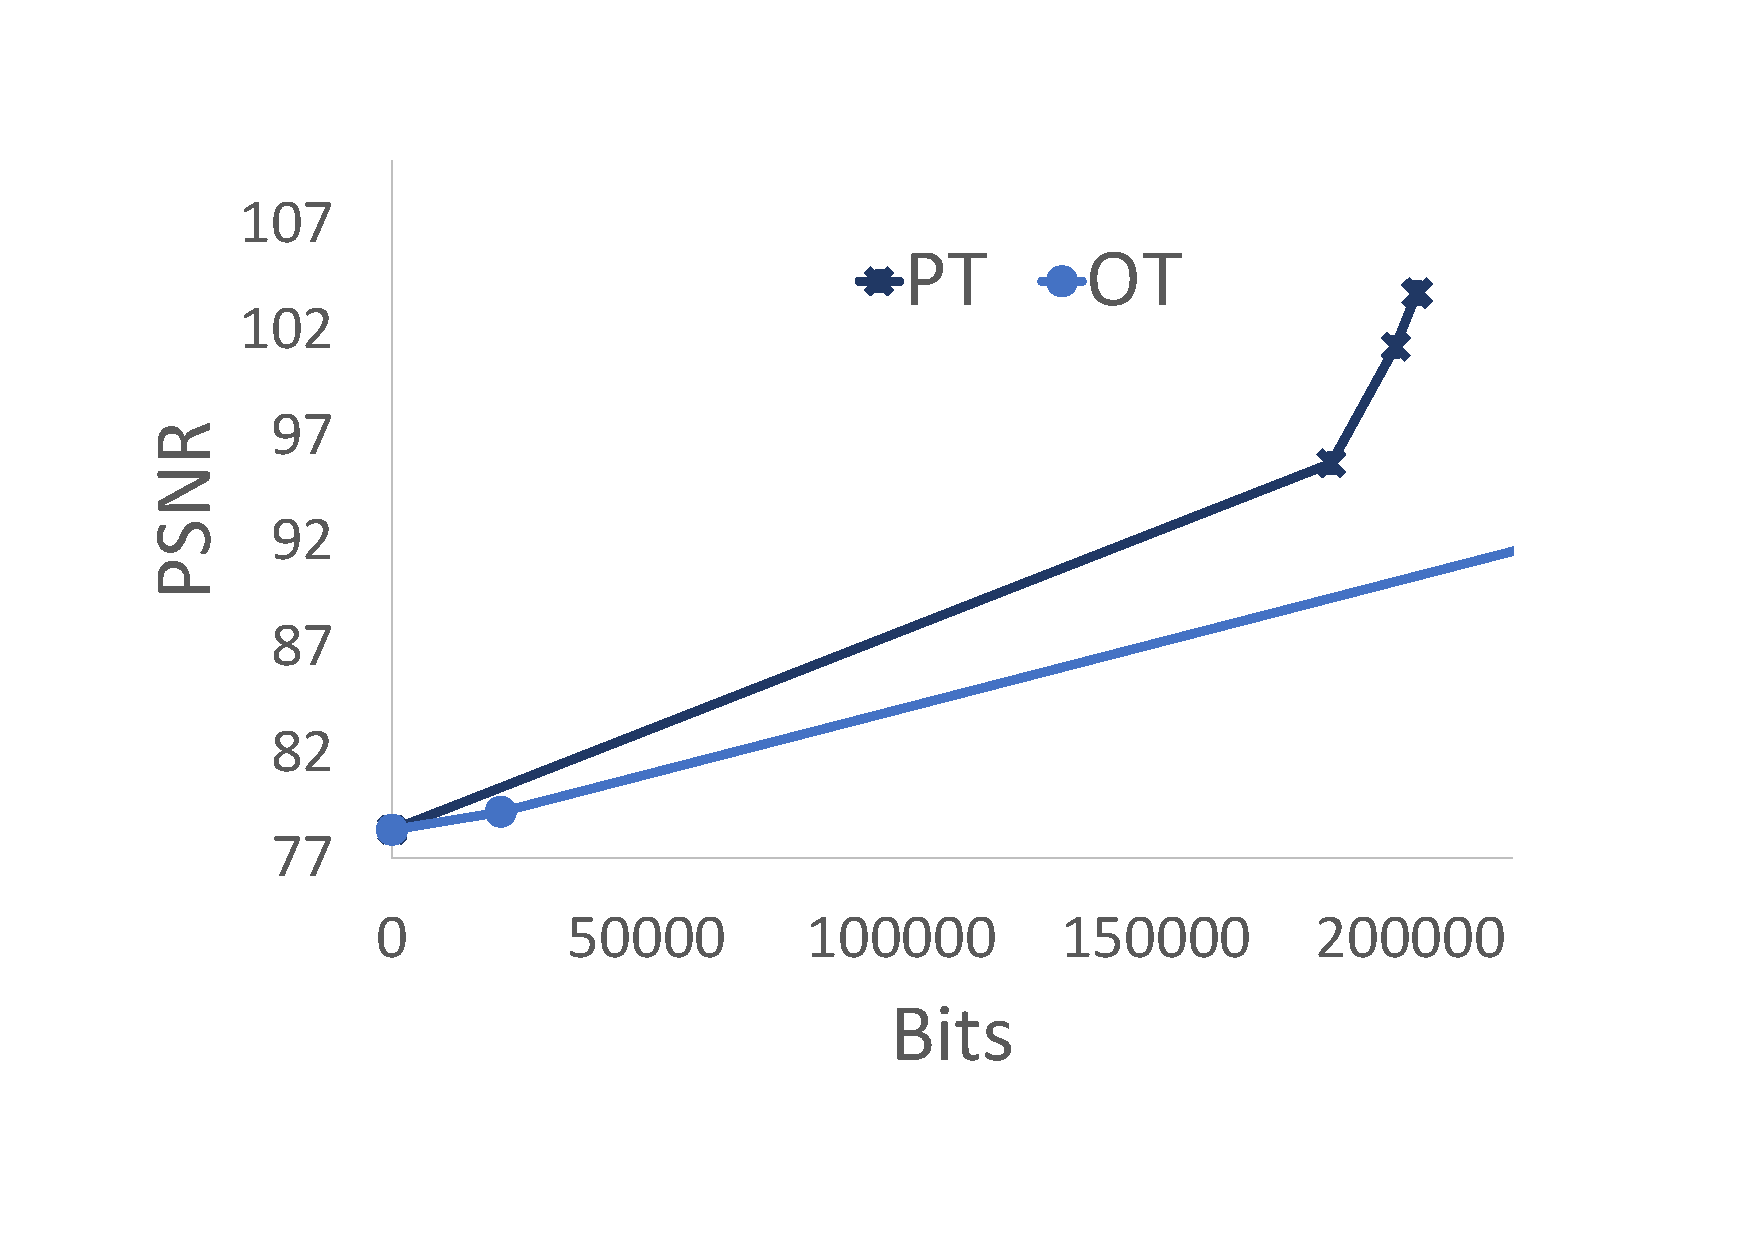
\includegraphics[width=4.0in]{images/results/compression/psnr1}
\caption{PSNR vs Bit-rate comparing the OT and Plane-Tree compression methods.}
\label{fig:3DReconCompression1}
\end{figure}

In conclusion, as in results comparing the Plane-Tree with state-of-the-art mesh compression algorithms, the Plane-Tree is shown to perform well and even outperform SOT and the generic octree data structures when compressing 3D data used in reconstructions. 
